% Preamble
\providecommand{\main}{../..}
\documentclass[class=article, crop=false]{standalone}

% Packages
\usepackage{\main/packages}

% Configurations
\graphicspath{{\main/images/}{images/}}
\cellspacetoplimit 4pt
\cellspacebottomlimit 4pt

% Document
\begin{document}
    \section{TOPIC 3 - Antenna Parameters}
    To describe the performance of an antenna, definitions of various parameters are neces-
    sary. Some of the parameters are interrelated and not all of them need be specified for
    complete description of the antenna performance. Parameter definitions will be given
    in this topic.\cite{BALANIS} \\

    \subsection{Radiation Patterns}
    \textbf{Antenna Radiation Pattern or Antenna Pattern:}\\
    \emph{The spatial distribution of a quantity that
    characterizes the electromagnetic field generated by an antenna.}

    \begin{figure}[h!]
        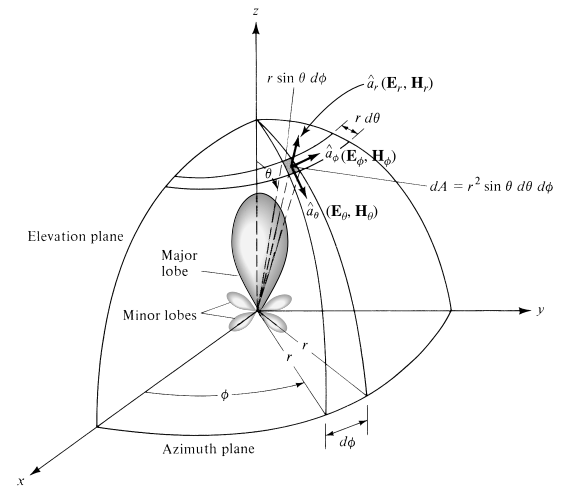
\includegraphics[width=\textwidth]{topics/3/radiation_patterns.png}
        \caption{Radiation Pattern Analysis \cite{BALANIS}}
        \label{fig:radiationpattern}
    \end{figure}

    \textbf{Types of patterns: }\\
    \cite{BALANIS}
    \begin{enumerate}
        \item \textbf{field pattern} (in linear scale) typically represents a plot of the magnitude of the
        electric or magnetic field as a function of the angular space.
        \item \textbf{power pattern} (in linear scale) typically represents a plot of the square of the
        magnitude of the electric or magnetic field as a function of the angular space.
        \item \textbf{power pattern} (in dB) represents the magnitude of the electric or magnetic field,
        in decibels, as a function of the angular space.
    \end{enumerate}

    \textbf{
        Radiation Pattern's lobes:
    }
    \begin{itemize}
        \item Major lobe
        \item Minor lobe
        \item Side lobe
        \item Back lobe
    \end{itemize}
    \begin{figure}[h!]
        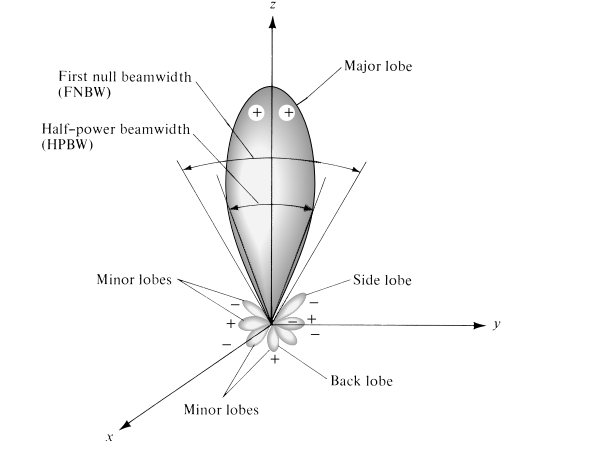
\includegraphics[width=\textwidth]{topics/3/lobes.png}
        \caption{Radiation Pattern Lobes \cite{BALANIS}}
        \label{fig:lobes}
    \end{figure}
    \begin{figure}[h!]
        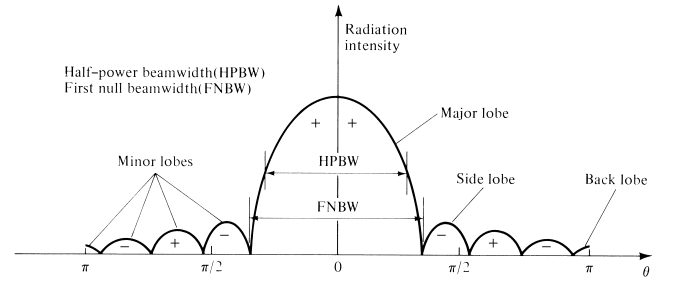
\includegraphics[width=\textwidth]{topics/3/lobes_intensity.png}
        \caption{Radiation Pattern Lobes Intensity \cite{BALANIS}}
        \label{fig:lobes_intensity}
    \end{figure}

    \textbf{Beamwidth:}\\
    \emph{
        the angular separation between two identical points on opposite side of the pattern maximum.
    }\\

    \textbf{Types of Beamwidth:}
    \begin{itemize}
        \item Half Power Beamwidth
        \item First Null Beamwidth
    \end{itemize}

    \textbf{Half Power Beamwidth Points on different patterns}
    \begin{itemize}
        \item field pattern at 0.707 value of its maximum.
        \item power pattern (in a linear scale) at its 0.5 value of its maximum.
        \item power pattern (in dB) at $- 3 \si{\decibel}$ value of its maximum.
    \end{itemize}
    \begin{figure}[h!]
        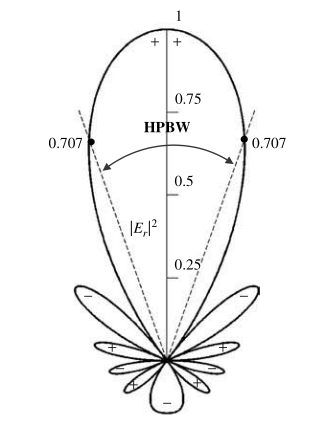
\includegraphics[width=0.3\textwidth]{topics/3/field_linear_scale.png}\hfill
        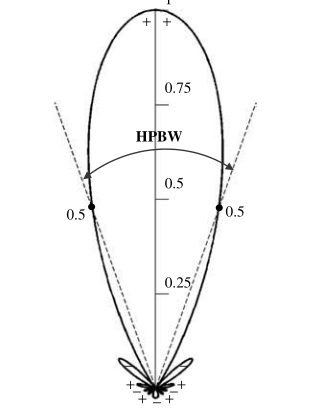
\includegraphics[width=0.3\textwidth]{topics/3/power_linear_scale.png}\hfill
        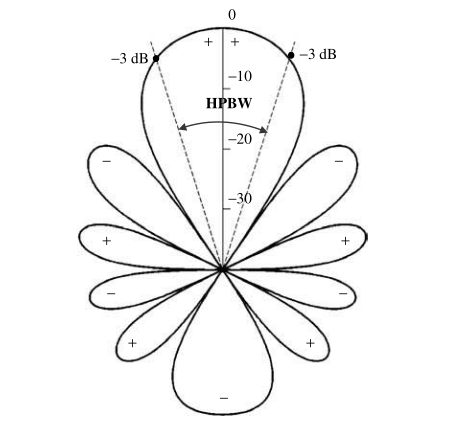
\includegraphics[width=0.4\textwidth]{topics/3/power_db_scale.png}
        \caption{Radiation Pattern Beamwidth \cite{BALANIS}}
        \label{fig:beamwidth}
    \end{figure}




\end{document}
